\section{Theory}


Let $\mathcal P$ be a polygon and $p(x, y) \in \mathcal P$ a guard. We are interested in computing the best direction for moving $p$ inside $\mathcal P$ such that the visibility area $Vis(p)$ increases. That is, exploring what would be a better position for $p$ such that $p$ ``sees more'' of the polygon $\mathcal P$. 

We can define $f(p)$ as the area seen by a guard $p$. Let $f'_i(p)$ be the local change in the area seen by guard $p$ around a reflex vertex $i$ of $\mathcal P$, as given by the derivative of $f$. Given all reflex vertices $i$, the total (global) change in the area seen by $p$ can be thus summed up to $f'(p) = \sum_i f'_i(p)$. Figure \ref{fig:sumf} offers an example for this case for a polygon $\mathcal P$ and its reflex vertices $r_1$ and $r_2$. The polygon $\mathcal P$ is guarded by $p$, and its position is modified to $p'$ by a small change $\partial y$. The visibility areas of $p$ become $f'_{r_1}$ and $f'_{r_2}$ around reflex vertices $r_1$ and $r_2$, respectively. In this way, the total change in the visibility area of $p$ becomes $f'(p) = f'_{r_1}(p) + f'_{r_2}(p)$.

Thus, $f(p)$ is the continuous objective function of The Art Gallery Problem. We can then use gradient descent as a method to optimise the objective function $f$. We will define below what the methodology of gradient descent is comprised of.

\begin{figure}[h!]
    \centering
    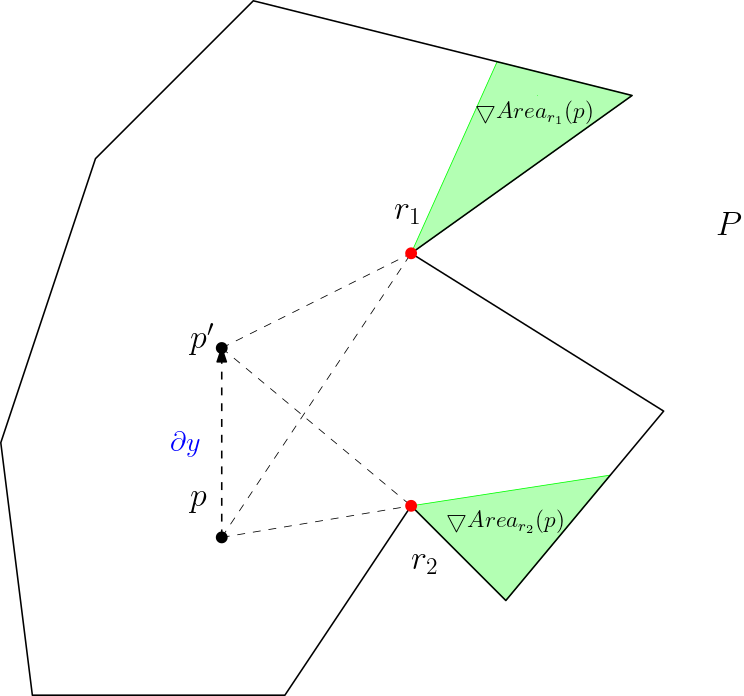
\includegraphics[width=0.4\textwidth]{sumf.png}
    \caption{Global change in the area seen by $p$ when moved by $\partial y$ to a new position $p'$.}
    \label{fig:sumf}
\end{figure}

Gradient descent is an iterative optimisation algorithm for finding the local maximum of a continuous differentiable function. The idea of gradient descent is to repeatedly move in the opposite direction of the gradient of the function at the current point. In this way, we can define $\bigtriangledown f$ to be the gradient of $f$. The gradient $\bigtriangledown f$ will then indicate the direction of the steepest descent for the objective function $f(p)$. 


% defining the gradient for computing the best change in the position of $p$.

Given that $f$ is a function that describes the visibility area of a point $p(x, y)$, we will first need to define how its gradient is computed. In order to simplify the gradient computation without losing generality, we will analyse the gradient by fixing one of the coordinates of $p$ and varying the other one. In this case, fixing the $x$-coordinate and varying the $y$-coordinate. As such, the computation of the gradient remains the same regardless of the rotation applied to the plane.


We will use the notation $\frac{\partial f}{\partial y}$ to denote the change in the visibility area $f(p)$ when the $y$-coordinate is modified by a small amount $\partial y \rightarrow 0$. Analogously, we will use $\frac{\partial f}{\partial x}$ to denote the small change in the $x$-coordinate of $p$. In this way, we define 

\begin{equation}
    \bigtriangledown f = (\frac{\partial f}{\partial x}, \frac{\partial f}{\partial y}) \label{eq:gradient}
\end{equation}

to be the gradient of $f$ given that $\mathcal P$ is guarded by a point $p(x, y)$. 

We will now create a canonical geometrical construction that will allow us to further define and compute $\bigtriangledown f$. In this case, we consider the normalised length of the gradient as $||\bigtriangledown f|| = 1$. This canonical construction is displayed in Figure \ref{fig:gradient}. We will then generalise this case to multiple reflex vertices and guards.

\begin{figure}[h!]
    \centering
    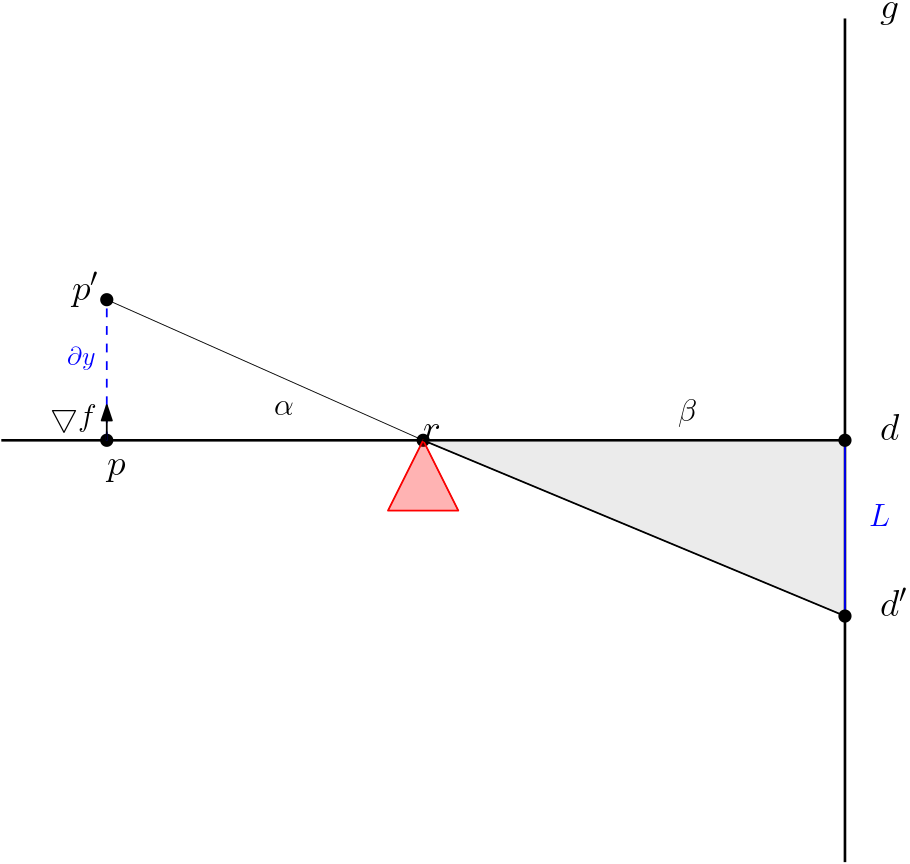
\includegraphics[width = 0.6\textwidth]{gradient2.png}
    \caption{Canonical gradient construction and for when the position of $p$ is varied by a small amount $\partial y$.}
    \label{fig:gradient}
\end{figure}

Let $g$ be a boundary line segment of $\mathcal P$, $r$ a reflex vertex inside $\mathcal P$ and $p$ a guard whose optimal position we are interested in. Let $\overline{pr} = \alpha$ be known. Additionally, let $d$ be the maximum point of visibility that $p$ can see behind $r$ on the line $g$. Let the distance between $r$ and $d$ be considered as $|\overline{rd}| = \beta$ known. 
% That is, the direction of the greatest increase of $f$. 

% We consider the case where there is only a positive change in the $y$ position of $p$. The case with a negative coordinate change would be analogous.


Let $\partial y$ be an extremely small change in the position of $p$. Call $p'$ this new position of $p$. The point $p'$ can see then up to a new maximum point $d'$ around $r$ on $g$. Let thus the distance between $d$ and $d'$ be $|\overline{dd'}| = L$. As such, $\triangle rdd'$ denotes the increase in the visibility area of $p$ when it moves to position $p'$. That is, the first derivative $f'(p)$ of $f$ will represent the change in the visibility area of $p$:

\begin{equation}
    \text{Area}_{\triangle rdd'} = f'_r(p). \label{eq:derivative}
\end{equation}

% Let $a''$ be the projection of $p'$ on $p''r$, and $a$ the projection of $a''$ on the line $pr$ such that the distance from $a$ to $r$ is $|\overline{ar}| = \alpha$. Take the distance between $p$ and $p'$ to be $x$. Since $a''$ is the projection of $p'$ on $pr$, then $|\overline{pp'}| = |\overline{aa''}| = x$.





% \subsection{Canonical Case}
% Consider the geometrical construction in Figure \ref{fig:gradient}. The construction was created for ease of computation, and the general case can be translated and rotated to this case.

% In this canonical case we will consider the situation where the gradient is normalised as $||\bigtriangledown f|| = 1$. 

We are now interested in computing how the area seen by guard $p$ increases given the change $\partial y$ in the position of $p$. The distances $||\overline{pr}|| = \alpha$ and $||\overline{rd}|| = \beta$ are known, so we aim at expressing the gradient $\bigtriangledown f$ through $\alpha$ and $\beta$. Since $\bigtriangledown f$ depends on the change in the coordinates of $p$, computing it is tightly connected to the change in the area of triangle $\triangle rdd'$. We will proceed to calculate the area of $\triangle rdd'$ below.
% We are now interested in computing the distances $|\overline{df}|, |\overline{aa'}|, |\overline{pp''}|, L$ such that we can compute the increase in the area seen by $p$ and thus the gradient $\bigtriangledown f$. The two triangle areas that need to be computed in order to do so are $A_{\triangle rdd'}$ and $A_{\triangle rdd''}$.

Given that triangles $\triangle rpp'$ and $\triangle rdd'$ are square triangles, their areas can be calculated as:

\begin{align}
    \text{Area}_{\triangle rpp'} &= \frac{\alpha \partial y}{2}, \label{eq:rpp}\\
    \text{Area}_{\triangle rdd'} &= \frac{\beta L}{2}. \label{eq:rdd}   
\end{align}


Given that $\overline{pp'}$ is parallel to $g$, we can use Thales's Theorem in triangles $\triangle rpp'$ and $\triangle rdd'$ to compute the length $L$: 

\begin{align}
    \frac{||\overline{pp'}||}{||\overline{dd'}||} &= \frac \alpha \beta \\
    \frac{\partial y}{L} &= \frac \alpha \beta  \label{eq:dxL} \\
    L &= \frac{\beta \partial y}{\alpha}. \label{eq:L}
\end{align}


% we can compute the length $L$: $$\frac{\text{Area}_{\triangle rdd'}}{\text{Area}_{\triangle rpp'}} = \frac{\frac{\beta L}{2}}{\frac{\alpha \partial x}{2}} = \frac{\beta L}{\alpha \partial x} \Rightarrow L = \frac{\partial x \beta}{\alpha}.$$

We are now interested in how areas $\text{Area}_{\triangle rpp'}$ and $\text{Area}_{\triangle rdd'}$ change depending on how $\alpha$ and $\beta$. That is, $\frac{\text{Area}_{\triangle rdd'}}{\text{Area}_{\triangle rpp'}}$ as a function of $\alpha$ and $\beta$: 

\begin{align}
    \frac{\text{Area}_{\triangle rpp'}}{\text{Area}_{\triangle rdd'}} \overset{(\ref{eq:rpp}), (\ref{eq:rdd})}{=} &\frac{\frac{\alpha \partial y}{2}}{\frac{\beta L}{2}} \\
    = &\frac{\alpha \partial y}{\beta L} \\
    \overset{(\ref{eq:dxL})}{=} &\frac{\alpha \alpha}{\beta \beta} \\
    \frac{\text{Area}_{\triangle rpp'}}{\text{Area}_{\triangle rdd'}} = &{(\frac \alpha \beta)}^2 \label{eq:rddrpp}
\end{align}

We can now express the area of $\triangle rdd'$ as only dependent on $\alpha, \beta$, the small position change $\partial y$ and the already known area of $\triangle rpp'$:

\begin{align}
    \text{Area}_{\triangle rdd'} \overset{(\ref{eq:rddrpp})}{=} &{(\frac \beta \alpha)}^2 \text{Area}_{\triangle rpp'} \\
    \overset{(\ref{eq:rpp})}{=} &{(\frac \beta \alpha)}^2 \frac{\alpha \partial y}{2} \\
    \text{Area}_{\triangle rdd'} = &\frac{\beta^2 \partial y}{2\alpha}. \label{eq:ardd}
\end{align}
% \end{align*}
% $$\frac{\partial f}{\partial x} = \frac{\text{Area}_{\triangle rdd'}}{\partial x}$$

Analogously, we can compute the change in the $y$-coordinate by rotating the plane with $90^\circ$ and follow the same steps. This procedure will result in

\begin{equation}
    \text{Area}_{\triangle rdd'} = \frac{\beta^2 \partial y}{2\alpha}. \label{eq:ardd2}
\end{equation}

Thus, the change in the visibility area $\text{Area}_{\triangle rdd'}$ of $p$ given the small change $\partial y$ in the position of $p$, and hence the gradient $\bigtriangledown f$ is 

\begin{align*}
    \bigtriangledown f \overset{(\ref{eq:gradient})}{=} &(\frac{\partial f}{\partial x} + \partial x, \frac{\partial f}{\partial y} + \partial y) \\
    \overset{(\ref{eq:derivative})}{=} &(\frac{\partial f}{\partial x} + \partial x, \frac{\text{Area}_{\triangle rdd'}}{\partial y} + 0) \\
    \bigtriangledown f \overset{(\ref{eq:ardd}), (\ref{eq:ardd2})}{=} &(\frac{\partial f}{\partial x} + \partial x, \frac{\beta^2}{2\alpha}). \\
\end{align*}

% Given that $pp''$ is parallel to $g$, we can use the Intercept Theorem to compute the lengths of the segments as follows:

% \begin{itemize}
%     \item in $\triangle raa'$, $\triangle rpp'$, with $aa' || pp'$: $$\frac{|\overline{pp'}|}{|\overline{dd'}|} = \frac{|\overline{pr}|}{|\overline{rd}|} \iff \frac{x}{|\overline{dd'}|} = \frac{1}{\beta} \Rightarrow |\overline{dd'}| = x\beta$$
    
%     $$\frac{|\overline{aa'}|}{|\overline{pp'}|} = \frac{\alpha}{1} = \frac{|\overline{aa'}|}{x} \Rightarrow |\overline{aa'}| = x\alpha$$

%     \item in $\triangle rpp''$, $\triangle raa''$, with $pp'' || aa''$: $$\frac{|\overline{aa''}|}{pp''} = \frac{|\overline{ar}|}{|\overline{pr}|} \iff \frac{x}{|\overline{pp''}|} = \frac{\alpha}{1} \Rightarrow |\overline{pp''}| = \frac{x}{\alpha}$$
    
%     \item in $\triangle rpp''$, $\triangle rdd''$, with $pp'' || dd''$: $$\frac{|\overline{pp''}|}{|\overline{dd''}|} = \frac{|\overline{pr}|}{|\overline{rd}|} \iff \frac{\frac{x}{\alpha}}{L} = \frac{1}{\beta} \Rightarrow L = \frac{x\beta}{\alpha}$$
% \end{itemize}

% Now the area of the square triangle $\triangle rdd''$ corresponding to the gradient $\bigtriangledown f$ can be computed as: $$\bigtriangledown f = \frac{|\overline{rd}||\overline{de}|}{2} = \frac{\beta L}{2} = \frac{\beta \frac{x\beta}{\alpha}}{2} = \frac{\beta^2x}{2\alpha}, ||x|| = 1$$


% \subsection{General Case}


% - we will only look at one coordinate (vary $y$), since varying $x$ is symmetrical, but rotated $90^\circ$

% - we will first look at a canonical situation $||\bigtriangledown f|| = 1, \alpha = \beta = 1$

% Let:

% - $f(p)$ - area seen by guard $p$

% - $f'_i(p)$ - the change in the area seen locally by guard $p$, as given by its derivative

% - $f'(p) = \sum_i f'_i(p)$ - the change in the area seen globally by guard $p$

% - $\bigtriangledown f = (\frac{\partial f}{\partial x}, \frac{\partial f}{\partial y})$ - the direction of the greatest increase of $f$

% - $r$ - reflex vertex

% - $p$ - guard whose position needs to be optimised

% - $|\overline{pr}| = 1$

% - $p', p''$ - the new positions of the guard where the $y$-coord is varied

    % - $|\overline{pp'}| = |\overline{aa''}| = x$

% - $\overline{ar} = \alpha, a \in \overline{pr}$ - additional guard construction

% - $\triangle rde$ - area seen by $p$

    % - $\triangle rdf$ - area seen by $p'$

% - $|\overline{rd}| = \beta$ - distance between reflex vertex and polygon boundary

% - $|\overline{de}| = L$

% Using the Intercept Theorem:

% - in $\triangle ra'a$, $\triangle rp'p$: $\frac{|\overline{pp'}|}{|\overline{df}|} = \frac{|\overline{pr}|}{|\overline{rd}|} = \frac{x}{|\overline{df}|} = \frac{1}{\beta} \Rightarrow |\overline{df}| = x\beta$

% - in $\triangle pp'r$, $\triangle aa'r$: $\frac{|\overline{aa'}|}{|\overline{pp'}|} = \frac{\alpha}{1} = \frac{|\overline{aa'}|}{x} \Rightarrow |\overline{aa'}| = x\alpha$

% - in $\triangle pp''r$, $\triangle aa''r$: $\frac{|\overline{aa''}|}{pp''} = \frac{|\overline{ar}|}{|\overline{pr}|} = \frac{x}{|\overline{pp''}|} = \frac{\alpha}{1} \Rightarrow |\overline{pp''}| = \frac{x}{\alpha}$

% - in $\triangle pp''r$, $\triangle rde$: $\frac{|\overline{pp''}|}{|\overline{de}|} = \frac{|\overline{pr}|}{|\overline{rd}|} = \frac{\frac{x}{\alpha}}{L} = \frac{1}{\beta} \Rightarrow L = \frac{x\beta}{\alpha}$

% Computing the area of the square triangle $\triangle rde$:

% - $A = \frac{|\overline{rd}||\overline{de}|}{2} = \frac{\beta L}{2} = \frac{\beta \frac{x\beta}{\alpha}}{2} = \frac{\beta^2x}{2\alpha}$